\documentclass{beamer}

\usepackage[utf8]{inputenc}
\usepackage[french]{babel}

%\usetheme{tb}
\definecolor{kugreen}{RGB}{66,103,104}
\definecolor{kugreenlys}{RGB}{86,157,160}
\definecolor{kugreenlyslys}{RGB}{165,165,165}
\definecolor{kugreenlyslyslys}{RGB}{242,242,242}
\setbeamercovered{transparent}
\mode<presentation>
{  \usetheme{PaloAlto}
  \usecolortheme[named=kugreen]{structure}
  \useinnertheme{circles}
  \usefonttheme[onlymath]{serif}
  \setbeamercovered{transparent}
  \setbeamertemplate{blocks}[rounded][shadow=true]
}

\title[Service Routière]{\textbf{Implémentation de Service de Collecte et de Stockage des Données sur une plateforme de services Routières}}
%\subtitle{Mémoire de projet de fin d'études}
\author{Moez Bouhlel \and Rihab Majdoub}
\author[Moez B. \and Rihab M.]{\textbf {Moez Bouhlel \and Rihab Majdoub\\[0.2cm] \footnotesize Sous la direction de: \\ Dr. Mohamed Mhiri \and M. Mohamed Amri}}
\institute{Faculté des Sciences de Sfax}
%\titlegraphic{
\includegraphics[width=2cm]{figures/logo-djagora}}
\logo{
\includegraphics[width=1.6cm]{./figures/fss-old}}
\date{05/06/2017}
\begin{document}
{
    \frame{\titlepage}
}

\begin{frame}
    \frametitle{Plan de la présentation}
    \tableofcontents[hideallsubsections]
\end{frame}

\AtBeginSection[]
{
  \begin{frame}
    \frametitle{Plan de la présentation}
    \tableofcontents[currentsection,hideothersubsections]
  \end{frame}
}

\section{Contexte de projet}
\begin{frame}
\frametitle{Organisme d'accueil}
\framesubtitle{Djagora Academy}
\begin{figure}
    
\includegraphics[width=.7\textwidth]{figures/logo-djagora.png}
\end{figure}
\end{frame}

\begin{frame}
    \frametitle{Présentation du projet}
    \framesubtitle{Équipe City Watch}
\begin{figure}
    
\includegraphics[width=.6\textwidth]{figures/logo-citywatch.jpg}
\end{figure}
\end{frame}

\begin{frame}
    \frametitle{Problématique}
    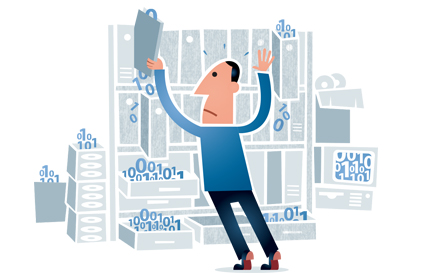
\includegraphics[width=.6\textwidth]{figures/datamanagement-issues.jpg}
    
\includegraphics[width=.32\textwidth]{figures/question.png}
\end{frame}

\begin{frame}
    \frametitle{Présentation du projet}
    \framesubtitle{Objectif}
    \begin{columns}
        \begin{column}{0.5\textwidth}
            \begin{figure}
                
\includegraphics[width=1\textwidth]{figures/logo-citywatch.jpg}
            \end{figure}
        \end{column}
        \begin{column}{0.5\textwidth}
            \begin{itemize}
                \item<1-> Collecte des données
                \item<2-> Analyse des données
                \item<3-> Valorisation des données
            \end{itemize}
        \end{column}
    \end{columns}
\end{frame}

\begin{frame}
    \frametitle{Présentation du projet}
    \framesubtitle{Architecture}
    \begin{figure}
        \centering
    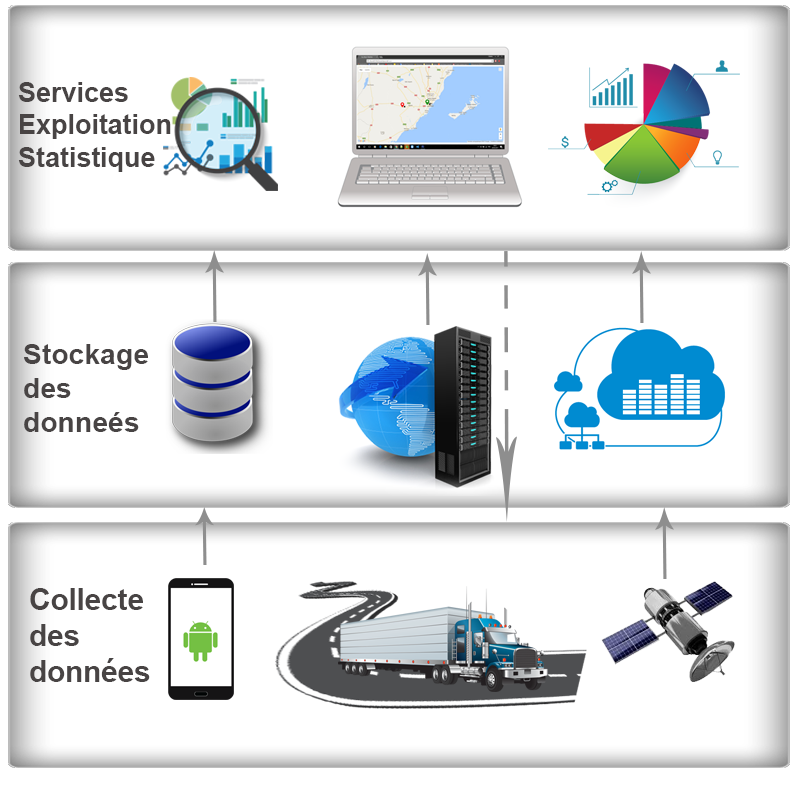
\includegraphics[width=.73\textwidth]{figures/citywatch-modules.png}
\end{figure}
\end{frame}

\section{Gestion projet selon Scrum}
\begin{frame}
    \frametitle{Pourquoi Scrum}
    \centering
    
\includegraphics[width=.7\textwidth]{figures/scrum-logo}
\end{frame}
\begin{frame}
    \frametitle{Méthodologie Scrum}
    \centering
    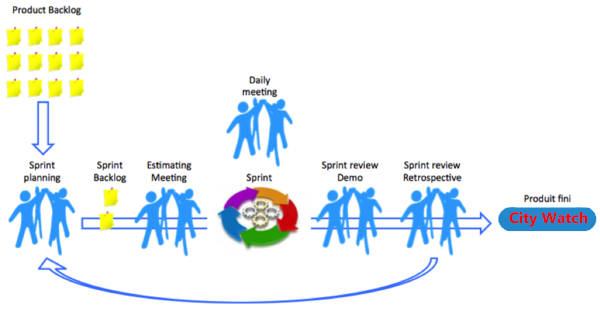
\includegraphics{figures/scrum-model}
\end{frame}

\section{Itération 1: Service Localisation}
\begin{frame}
    \frametitle{But de l'itération}
    \begin{itemize}
        \item<1-> Application mobile qui détecte la position géographique.
        \item<2-> Page web pour afficher la dernière position.
    \end{itemize}
\end{frame}
\begin{frame}
    \frametitle{Diagramme de cas d'utilisation}
    \begin{figure}
        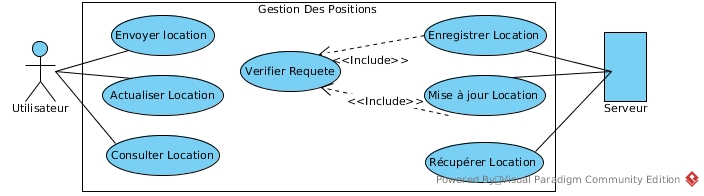
\includegraphics[width=1\textwidth]{./diagrams/sprint1-webservices-usecase.jpg}
    \end{figure}
\end{frame}
\begin{frame}
    \frametitle{Diagramme de séquence}
    \begin{figure}
        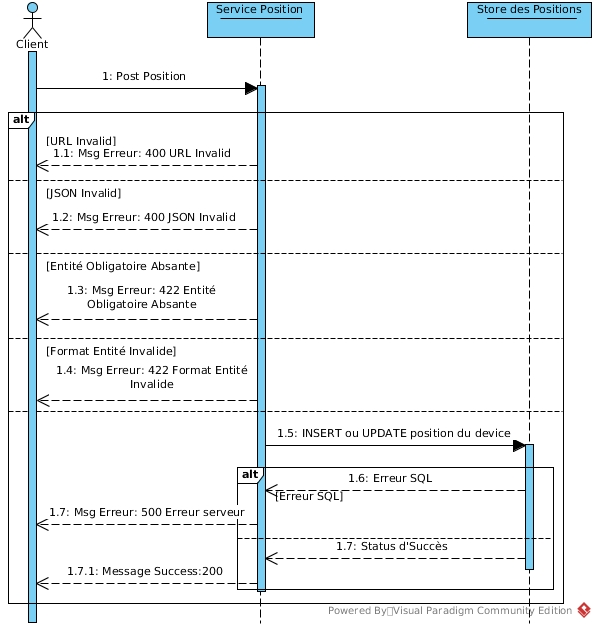
\includegraphics[width=0.7\textwidth]{./diagrams/sprint1-webservices-post-sequence.jpg}
    \end{figure}
\end{frame}
\begin{frame}
    \frametitle{Produit de l'itération}
    \begin{figure}
        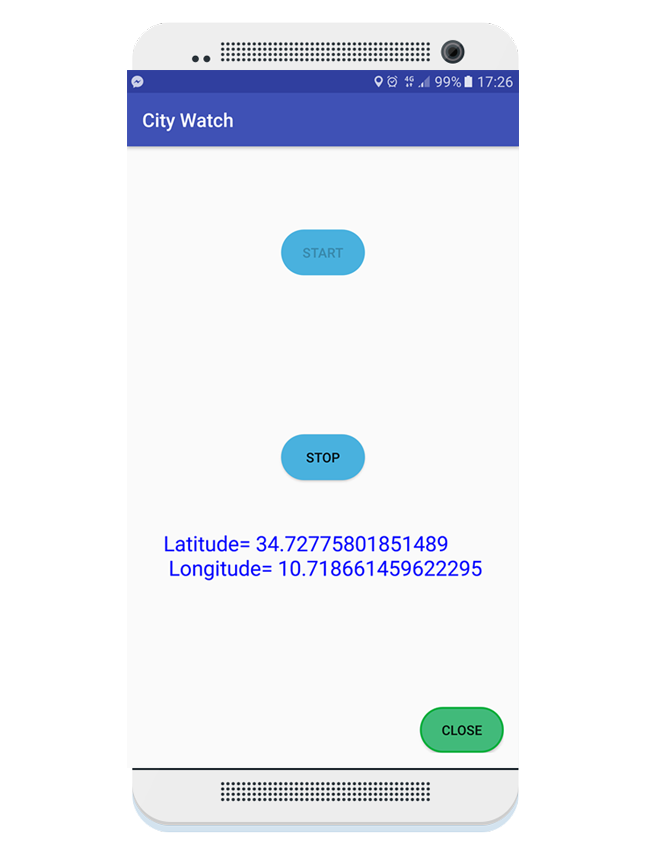
\includegraphics[width=0.3\textwidth]{./figures/sprint1-android-screenshot}
        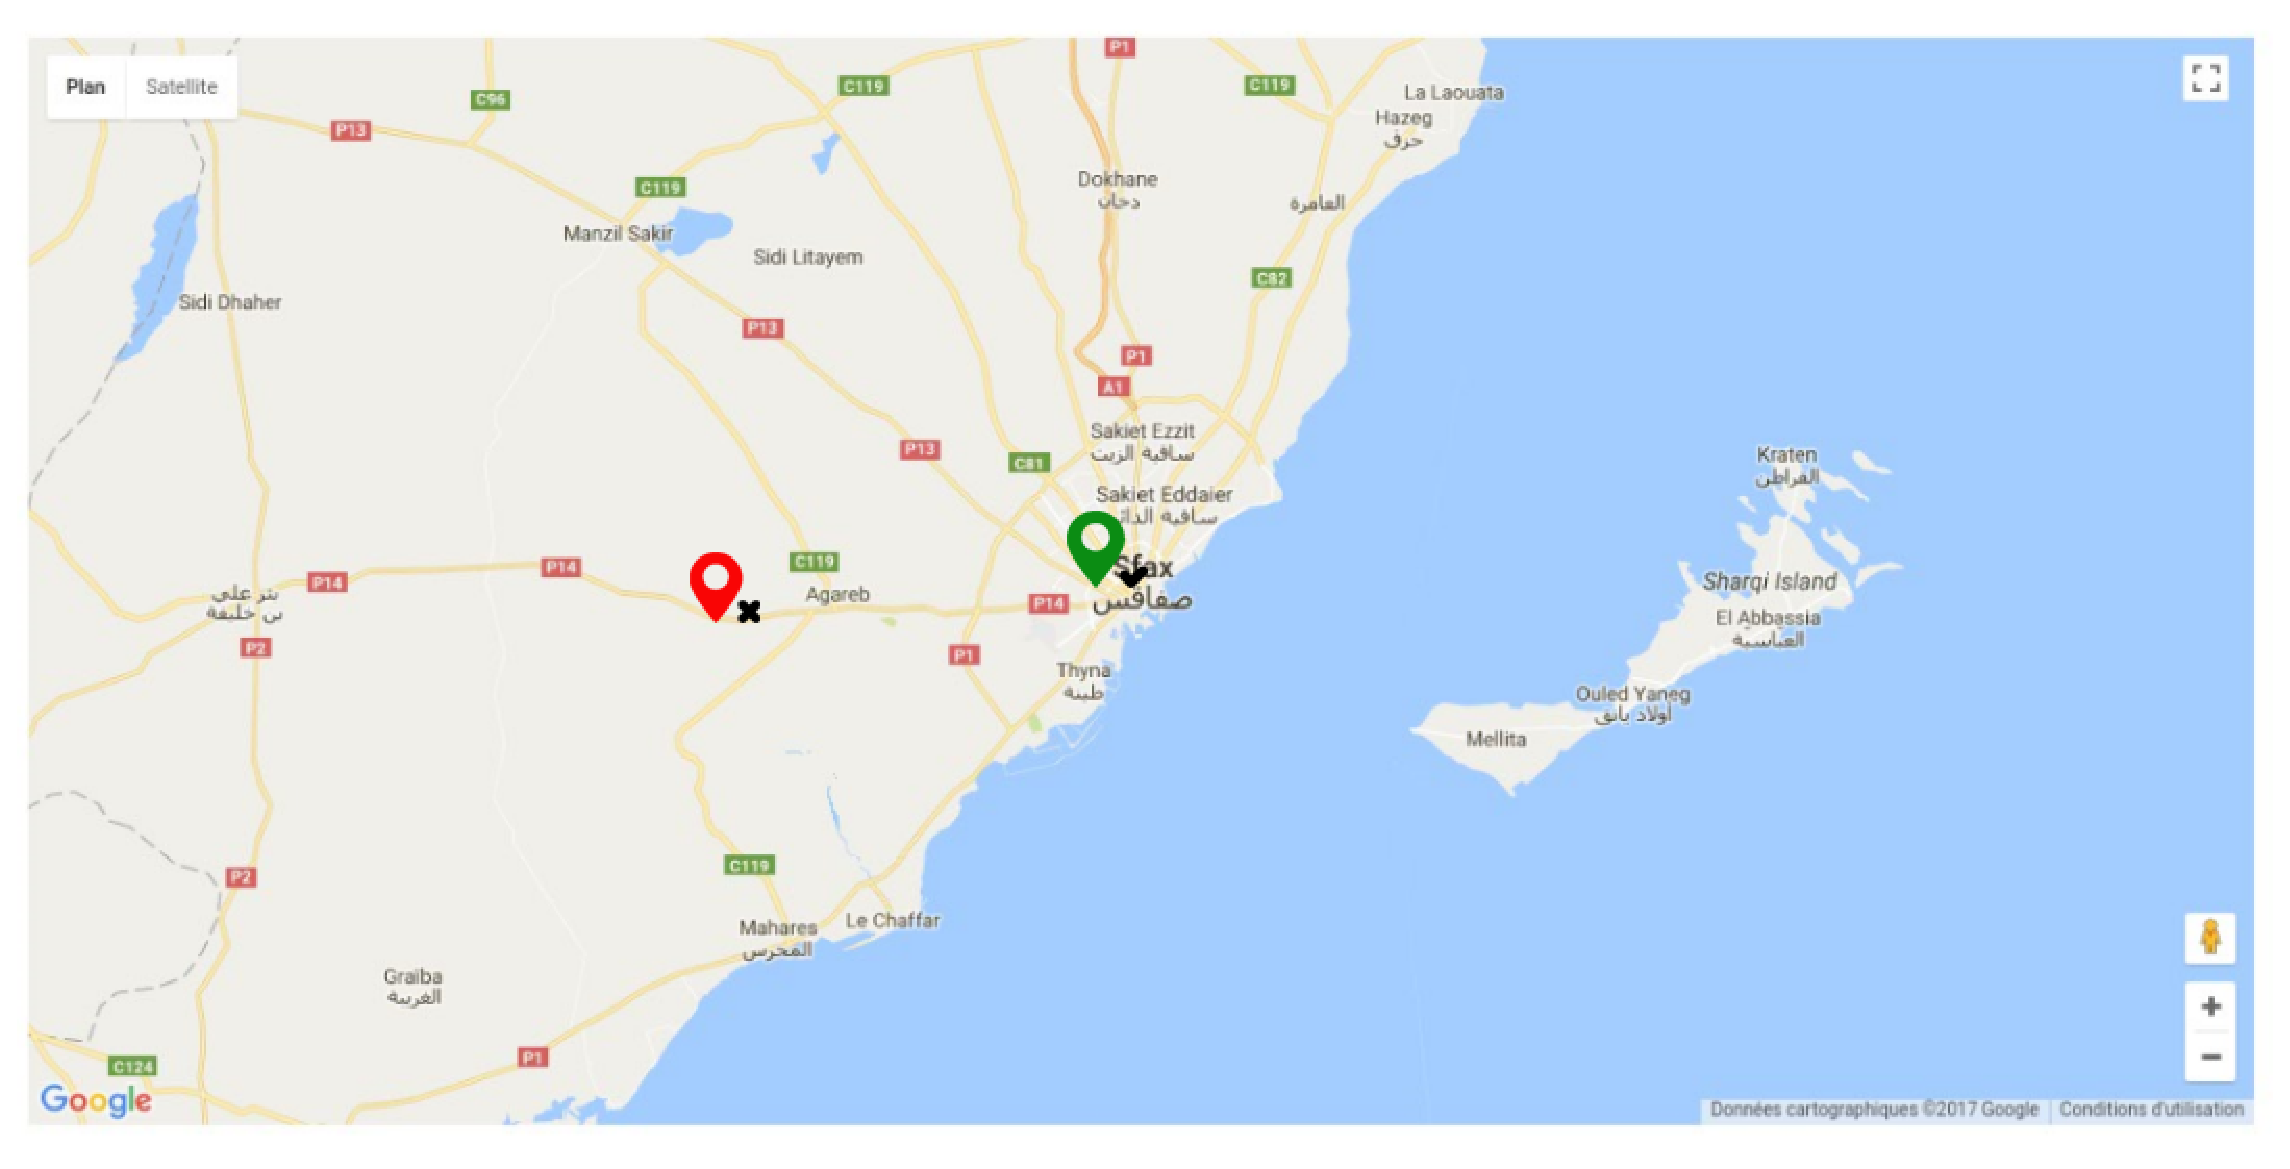
\includegraphics[width=0.7\textwidth]{./figures/sprint1-dashboard-screenshot}
    \end{figure}
\end{frame}

\section{Itération 2: Gestion des Rapports}
\begin{frame}
    \frametitle{But de l'itération}
    \begin{itemize}
        \item<1-> Déclaration des rapports.
        \item<2-> Détecte des secousses et ralentisseurs.
        \item<3-> Consultation des trajectoires, des rapports, des secousses et des ralentisseurs.
    \end{itemize}
\end{frame}
\begin{frame}
    \frametitle{Diagramme de cas d'utilisation}
    \begin{figure}
        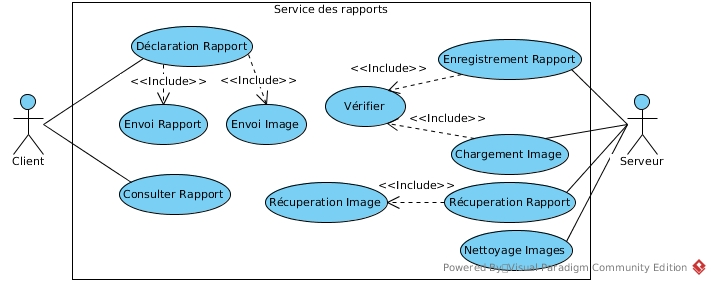
\includegraphics[width=\textwidth]{./diagrams/sprint2-webservices-report-usecase}
    \end{figure}
\end{frame}
\begin{frame}
    \frametitle{Diagramme de séquence}
    \begin{figure}
        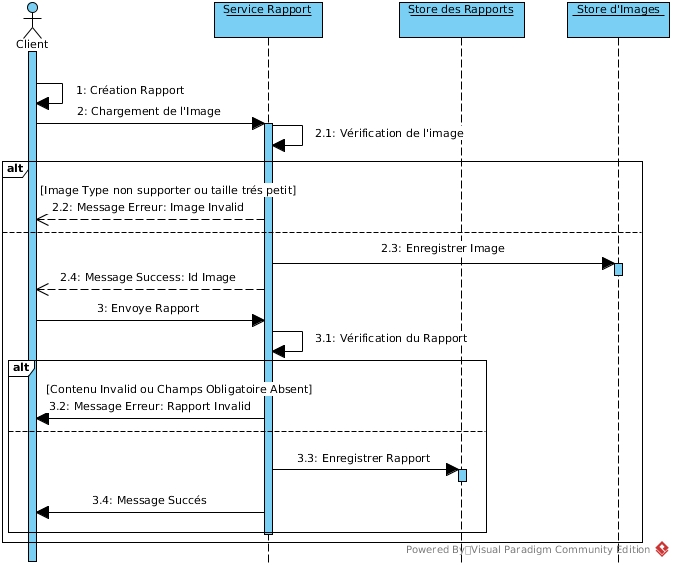
\includegraphics[width=.8\textwidth]{./diagrams/sprint2-webservices-report-post-sequence}
    \end{figure}
\end{frame}
\begin{frame}
    \frametitle{Produit de l'itération}
    \begin{figure}
        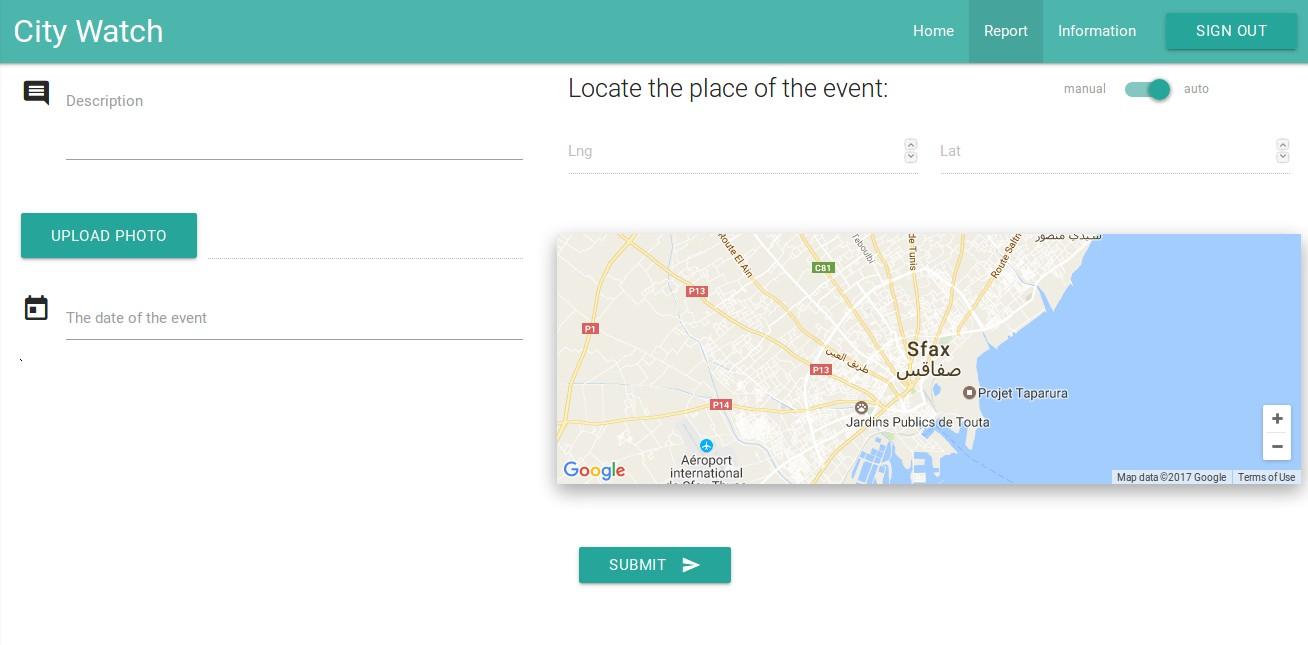
\includegraphics[width=0.45\textwidth,height=4cm]{./figures/sprint2-rapport-screenshot1}
        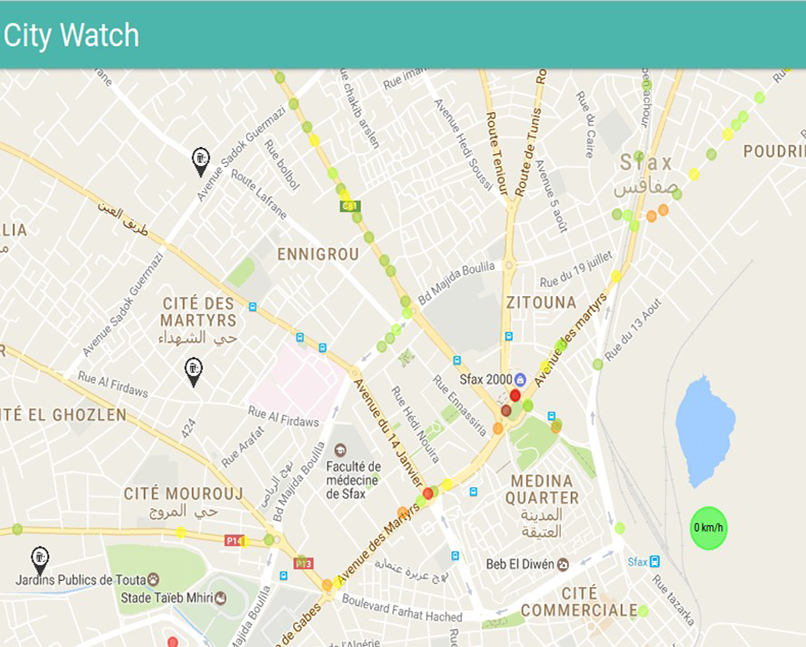
\includegraphics[width=0.5\textwidth]{./figures/sprint2-dashboard-screenshot2}
    \end{figure}
\end{frame}

\section{Itération 3: Authentification}
\begin{frame}
    \frametitle{But de l'itération}
    \begin{itemize}
        \item<1-> Détecte et projection de vitesse moyenne, d'état du réseau cellulaire.
        \item<2-> Authentification.
        \item<3-> Business Intellegence.
    \end{itemize}
\end{frame}
\begin{frame}
    \frametitle{Diagramme de cas d'utilisation}
    \begin{figure}
        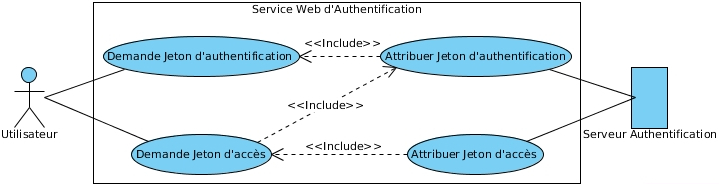
\includegraphics[width=\textwidth]{./diagrams/sprint3-webservices-oauth-usecase}
    \end{figure}
\end{frame}
\begin{frame}
    \frametitle{Diagramme de séquence}
    \begin{figure}
        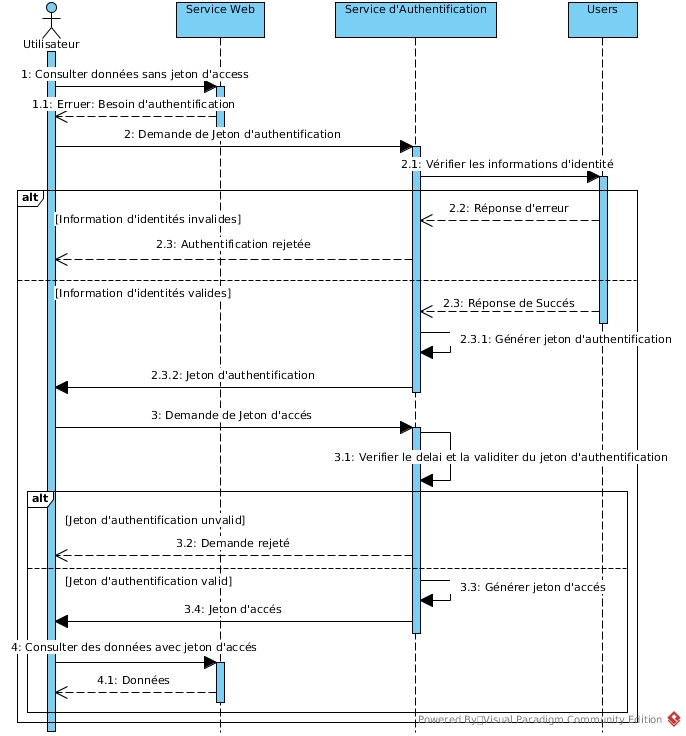
\includegraphics[width=.65\textwidth]{./diagrams/sprint3-webservices-oauth-sequence}
    \end{figure}
\end{frame}
\begin{frame}
    \frametitle{Produit de l'itération}
    \begin{figure}
        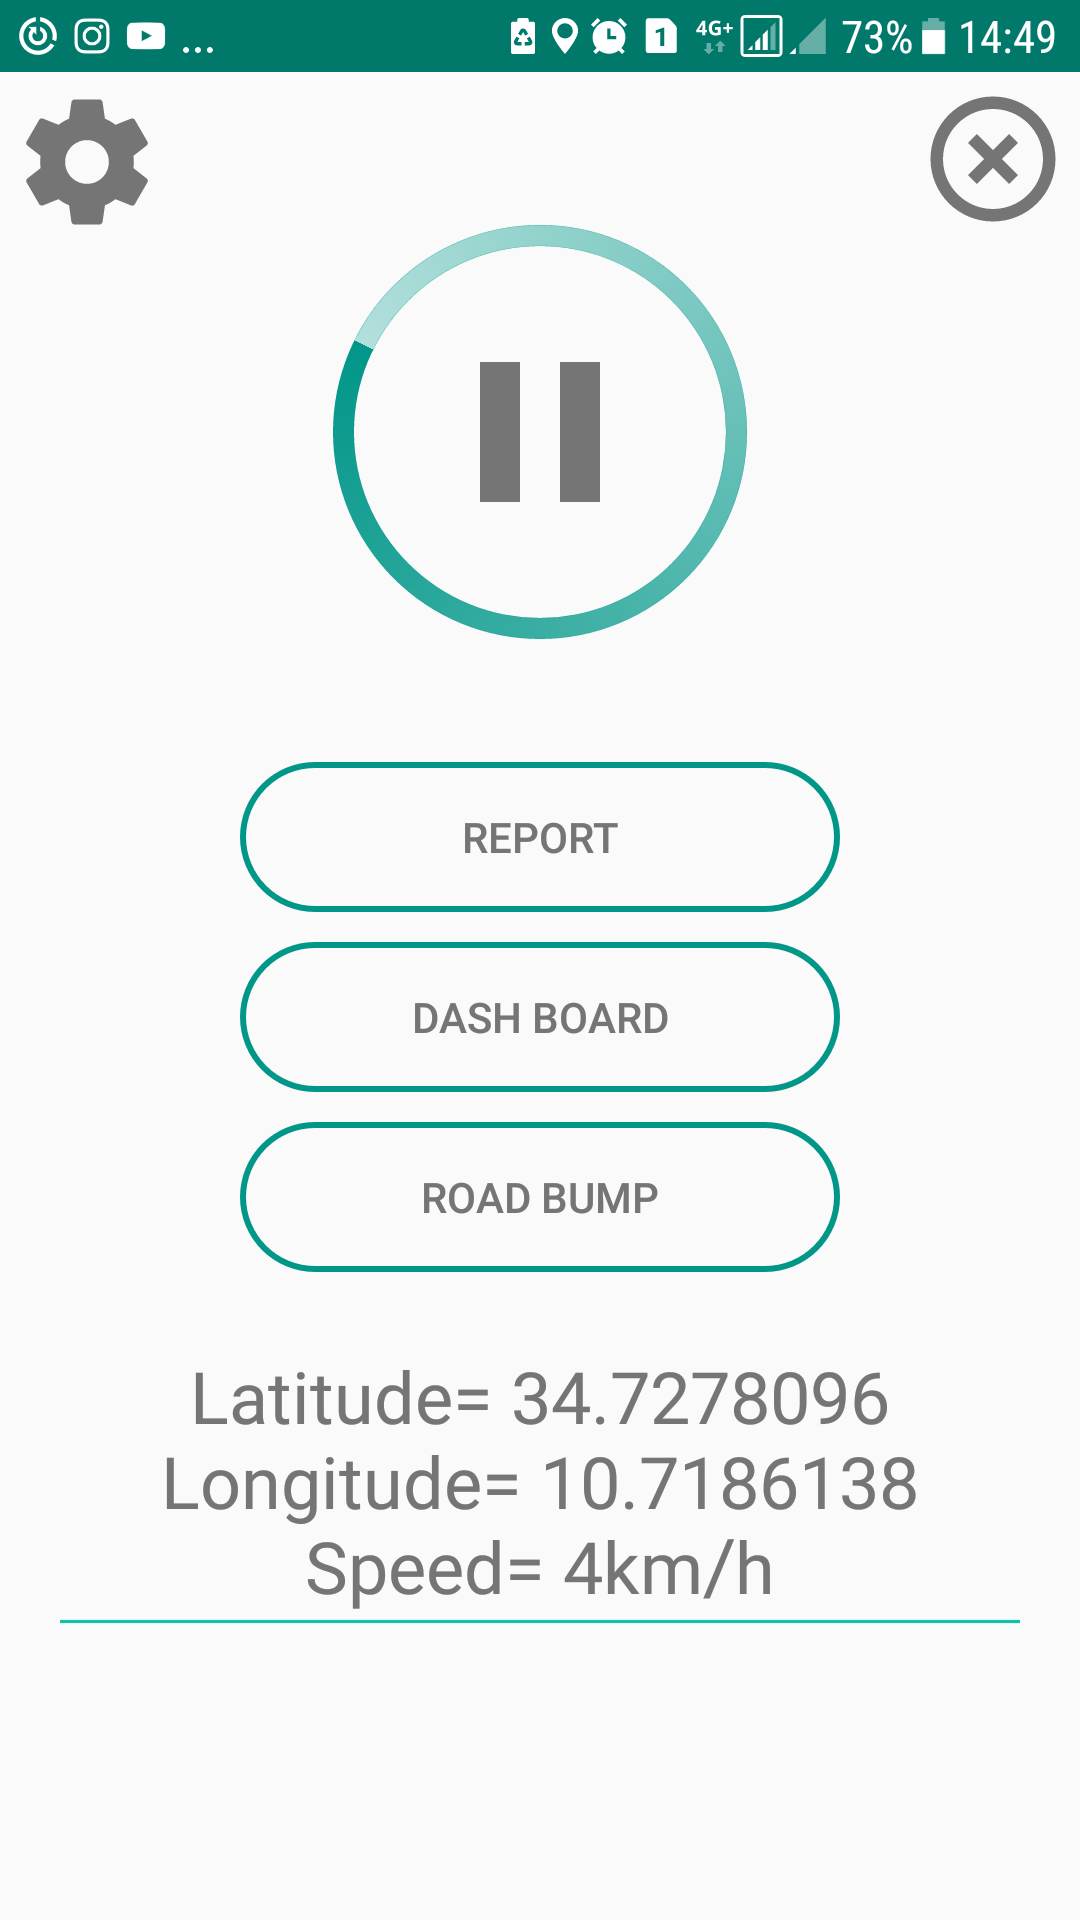
\includegraphics[width=0.35\textwidth]{./figures/sprint3-android-screenshot2}
        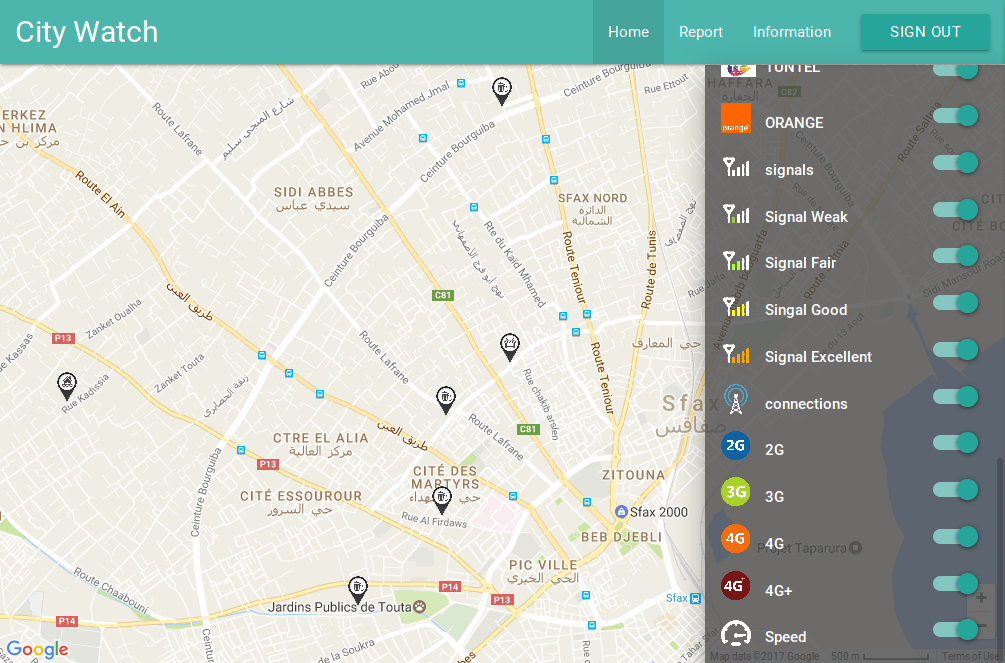
\includegraphics[width=0.65\textwidth]{./figures/sprint3-dashboard-screenshot1}
    \end{figure}
\end{frame}

\section{Réalisation}

\begin{frame}
\frametitle{Technologies utilisées}
\end{frame}
\begin{frame}
    \begin{center}
        \textbf{\Huge Démo}
    \end{center}
\end{frame}

\section{Conclusion \& Perspectives}
\begin{frame}
    \frametitle{Conclusion}
\end{frame}

\begin{frame}
    \frametitle{Perspectives}
\end{frame}

\end{document}
